\section{Task3. Pricing Strategy}

After studying the characteristics and relationship between the several indexes, we begin to investigate what an intelligent pricing strategy \parencite{psgxr} \parencite{wtl}should be like. In this section, we first value the rationality of the existing pricing strategy and then design a new dynamic pricing strategy based on what we have done before. At last, we also make a rationality test of the new pricing strategy, which proves to be effective.

\subsection{Task3(1). Rationality Test of the Existing Pricing Strategy}

In this section, we are going to test the rationality of the existing pricing strategy.

At first, We assume a simple pricing strategy: the one that keeps a stable freight rate. The revenue produced by this simple strategy will be used as a baseline to measure the rationality of other strategies. 

To calculate the total revenue, we first make efforts to simulate the sales volume. Take the flow direction of Yingkou-Shantou in the peak season as an example. We calculate the average market index of the flow direction through the way same as section 4.2.2 and then use the average to allocate the sales volume with initial value.

We dynamically adjust the sales volume fluctuation based on the lag time we have done in section 4.2.1 according to freight rate. At the same time, we change the freight rate as long as the space utilization reaches the threshold value according to the existing strategy of Company X. Then we compose the sales volume and freight rate to get the whole revenue, which is denoted as $Revenue_{Existing}$.

Similarly, we use the same technique to calculate the revenue of the simple pricing strategy of Company X, which is denoted as $Revenue_{Basic}$. We denote the ratio as the rationality through 

\begin{equation*}
    Rationality_{Existing} = \frac{Revenue_{Existing}}{Revenue_{Basic}}
\end{equation*}

The bigger the ratio is, the more rational the pricing strategy is.

\begin{figure}[H]
    \centering
    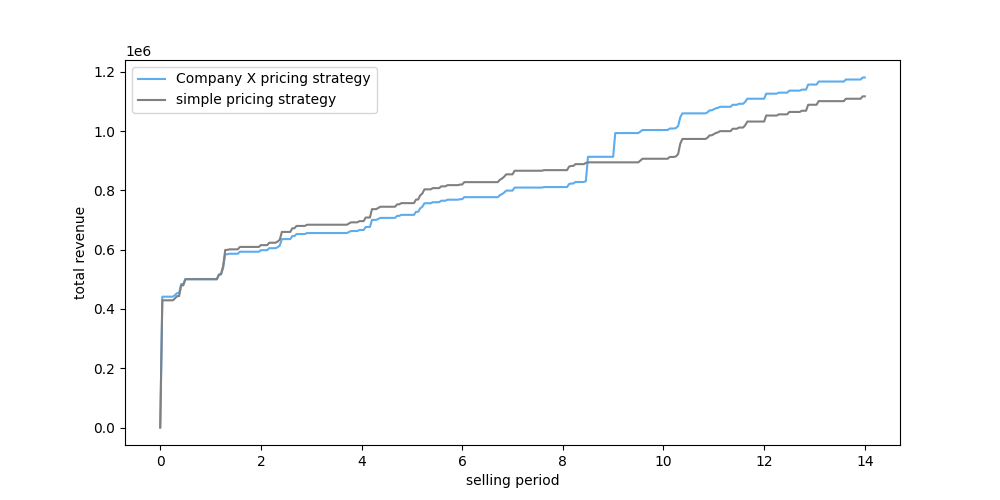
\includegraphics[scale=0.5]{Chapter-Mock/images-Mock/3_1.png}
    \caption{Rationality test of the existing pricing strategy.}
    \label{fig:Mock-Rationality-Existing}
\end{figure}

Seeing from the figure \ref{fig:Mock-Rationality-Existing}, we can conclude that the existing pricing strategy of the shipping company X has its rationality.

\subsection{Task3(2). Design of the Intelligent Pricing Strategy}

In order to achieve the goal of the shipping company X to maximize the revenue, we start to design and formulate a smarter and more reasonable pricing strategies.

Our design is shown in the following steps.
\begin{enumerate}[\quad\bf1.]
\item We make an assumption in our pricing strategy firstly, which is the entire selling periods of different SVVDs are all the same 14 days. Although the sales period of each voyage is different, we follow the 14-day sales period under popular conditions, which makes our model universal. Then we divide the 14-day sales period into $n$ extremely small sales time units.

\item Simple explanation for the pricing strategy

\hspace{1em}
We denote current freight Rate ($CFR$) and changing rate ($CR$) as two basic indexes to measure and change the freight rate. The notation of $CFR$ tends to directly show the current freight rate, which can be seen by customers. Meanwhile, $CR$ is defined to control the change of the freight rate precisely and timely, which is calculated by the pricing strategy and cannot be seen by customers.

\hspace{1em}
We suppose that the pricing strategy will automatically calculated the $CR$ in each sales time units based on the data and then change the $CFR$ according to the formula and objective function that we set in the pricing strategy.

\item Details and Formulas in the pricing strategy

\hspace{1em}
As for $CFR$, we set an initial freight rate, which is denoted as $CFR_0$. Now that $CFR$ will change in a stable interval, we denote the $CFR$ in the $i^{th}$ time unit  as $CFR_i$, where $i\in\{0,1,\dots,n \}$. Similarly, the $i^{th}$ $CR$ is also denoted as $CR_i$. However, the value of $CFR_0$ needs further discussion. Observing historical data, we know that freight rate fluctuations are small fluctuations within a certain range.So we average the historical price to determine the initial price $CFR_0$.

\hspace{1em}
In terms of $CR$, we combine what we have done together to form a complete influencing factor system.

\hspace{1em}
Firstly, we determine how booking habits affect the $CR$. As we have discussed in Task 2(2), plenty waybill orders often come after decrease in freight rate with lags within 17 hours. This may implies the sensitivity of customers to the freight rate decrease. For example, customers in one flow direction may immediately book the container after noticing a slight decrease on the freight rate, while customers in the other flow direction may patiently wait to book the container until the decrease achieves their ideal level. Such behavior difference can be measured by the lag hours in Task2(2) Granger Cause Test, and here we denote the lag hours as $time_{lag}$. From Task 2(2), we have ten lag hours from $time_{lag}^1$ to $time_{lag}^{10}$ and we can find the maximum which is $time_{lagmax}$. Then we can get the first influencing factor, which we denote as 
\begin{equation*}
    SSTV_i = \frac{time_{lag}^i}{time_{lagmax}}
\end{equation*}
where $i = 1,2,\dots,10$. $SSTV_i$ implies customers' sensitivity to freight rate decrease in the $i^{th}$ flow direction. The bigger $SSTV_i$ is, the more likely it is for customers to wait longer time for a bigger freight rate decrease.

\hspace{1em}
Secondly, we consider the effect of space utilization rate. It is easy to know that higher space utilization rate brings higher revenue. We decide to use $CSUR_i^k$ to symbolize the current space utilization rate of the $k^{th}$ flow direction in the $i^{th}$ selling period. We can get $CSUR_i^k$ through 
\begin{equation*}
    CSUR_i^k = \frac{CurrentUsed}{Total}
\end{equation*}
where $CurrentUsed$ is the number of used containers until the $i^{th}$ selling period and $Total$ is the entire container number of $k^{th}$ flow direction. If $CSUR$ is too low, it will be urgent for the company to decrease the freight rate to appeal to more customers.

\hspace{1em}
Thirdly, we talk about the influence of the selling period stage. Suppose we divide the 14-day-long selling period into $N$ small intervals. Then we can get the current selling period stage through 
\begin{equation*}
    CSPS_i^n = 1-\frac{i}{N}
\end{equation*}
where $i = 1,2,\dots,N$ and $n = 1,2,\dots,10$. With the approaching of departure time, $CSPS$ will become smaller to 0 and means that it is more necessary to care about the empty container.

\hspace{1em}
Fourth, we take the market demand into account. In the way similar to the operation on booking habits, we calculate the ratio between the market demand of the $i^{th}$ selling period $MD_i$ and the overall maximum market period $MD_max$. Then we get the current market demand through 
\begin{equation*}
    CMD_i = \frac{MD_i}{MD_max}
\end{equation*}


\item Construction of $CR$ with the influencing factors 

\hspace{1em}
In the former part, we have discussed the four indexes that affect $CR$ and analyze them to get the same principle that the bigger the index is, the less likely it is for the shipping company to decrease the freight rate. Since these four indexes have the same evaluation meaning, we use \textbf{Analytic Hierarchy Process} (AHP) to decide their weights and achieve a new index $CR$.

\hspace{1em}
To begin with, construct the judgment matrix of $CR-P$: Compare the four factors in pairs to get the judgment matrix (see in Figure \ref{fig:Judgment matrix of CR-P}).

% \begin{table}[H]
%     \renewcommand\arraystretch{2}   %%控制行间距
%     \centering
%     \begin{tabular}{ccccc}    %%三列均左对齐
%         \toprule  %%表格横线加粗
%         \specialrule{0em}{2pt}{2pt}    %%添加透明线控制行高
%          & $SSTV$ & $CSUR$ & $CSPS$ & $CMD$ \\
%         \specialrule{0em}{2pt}{2pt}    %%添加透明线控制行高
%         \hline
%         \specialrule{0em}{1pt}{1pt}    %%添加透明线控制行高
%         $SSTV$ & 1.0000 & 0.5000 & 4.0000 & 0.2500 \\
%         $CSUR$ & 2.0000 & 1.0000 & 2.0000 & 0.5000 \\
%         $CSPS$ & 0.2500 & 0.5000 & 1.0000 & 0.2000 \\    
%         $CMD$ & 4.0000 & 2.0000 & 5.0000 & 1.0000 \\
%         \specialrule{0em}{1pt}{1pt}    %%添加透明线控制行高
%         \bottomrule
%     \end{tabular}
%     \caption{Judgment matrix of $CR-P$.}
%     \label{tbl:Judgment matrix of CR-P}
% \end{table}

\begin{figure}[H]
    \centering
    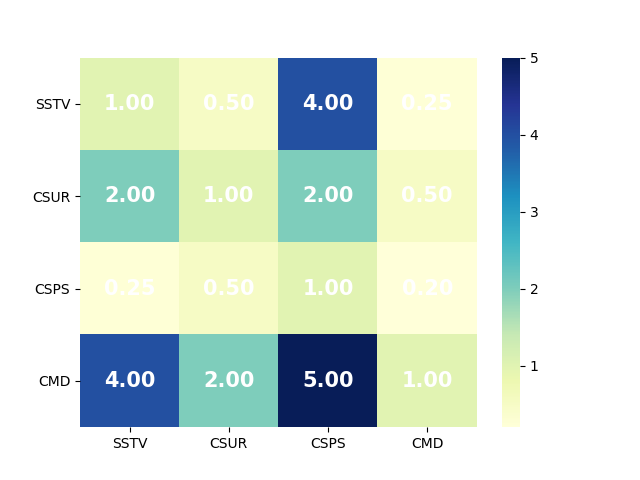
\includegraphics[scale=0.8]{Chapter-Mock/images-Mock/AHP.png}
    \caption{Judgment matrix of $CR-P$.}
    \label{fig:Judgment matrix of CR-P}
\end{figure}

\hspace{1em}
%%计算特征值，权重向量
%%代码见python
After that, it is easy to solve the eigenvalues of the matrix $CR-P$ and get the weight vector is $\omega_i = {(0.1701,0.2406,0.0805,0.5088)}^T$.

\hspace{1em}
Now we make the consistency check.

\hspace{1em}
Since the consistency index $CI = \frac{\lambda_{max}-n}{n-1}$ and the consistency ratio $CR = \frac{CI}{RI}$, where $RI$ is only relative to the matrix size (see in Table \ref{tbl:Mock-The value of RI}).

\hspace{1em}
By calculating, we get $CR = 0.0786<0.1$, which passes the consistency check.

%%The value of RI
\begin{table}[H]
    \renewcommand\arraystretch{2}   %%控制行间距
    \centering
    \begin{tabular}{ccccccccc}    %%三列均左对齐
        \toprule  %%表格横线加粗
        \specialrule{0em}{2pt}{2pt}    %%添加透明线控制行高
        matrix size & 2 & 3 & 4 & 5 & 6 & 7 & 8 & 9 \\
        \specialrule{0em}{2pt}{2pt}    %%添加透明线控制行高
        \hline
        \specialrule{0em}{1pt}{1pt}    %%添加透明线控制行高
        $RI$        & 0 & 0.58 & 0.90 & 1.12 & 1.24 & 1.32 & 1.41 & 1.45  \\
        \specialrule{0em}{1pt}{1pt}    %%添加透明线控制行高
        \bottomrule
    \end{tabular}
    \caption{The value of $RI$.}
    \label{tbl:Mock-The value of RI}
\end{table}

\hspace{1em}
To conclude, we can get the following $CR$ formula as 
\begin{equation*}
    CR = 0.1701\times SSTV+0.2406\times CSUR+0.0805\times CSPS+0.5088\times CMD
\end{equation*}

\item How $CR$ control the change of $CFR$

\hspace{1em}
After the data practice, we find the most intelligent pricing strategy with several indexes determined to maximize the revenue.

\hspace{1em}
For each selling period, we first calculate the present $CR$ and determine the freight rate change through the following way:

We design two different proposals to tackle different pricing strategy of peak season and off season.

\hspace{1em}
As for the $i^{th}$ selling period in the peak season,
\begin{equation*}
    CFR_{i+1} = \begin{cases}
    CFR_i+50\times\frac{CR_i-0.4}{0.4} & , \text{if } CR \geq 0.4; \\
    CFR_i-100\times\frac{0.4-CR_i}{0.4} & , \text{if } CR < 0.4.
    \end{cases}
\end{equation*}

\hspace{1em}
Similarly, the formula in the off season is
\begin{equation*}
    CFR_{i+1} = \begin{cases}
    CFR_i+20\times\frac{CR_i-0.6}{0.6} & , \text{if } CR \geq 0.6; \\
    CFR_i-150\times\frac{0.6-CR_i}{0.6} & , \text{if } CR < 0.6.
    \end{cases}
\end{equation*}
\hspace{1em}
To directly show the principle of our intelligent pricing strategy, we make the following framework of our algorithm in Figure \ref{fig:Intellignet pricing system}.

\begin{figure}[H]
    \centering
    %\vspace{-0.8cm}
    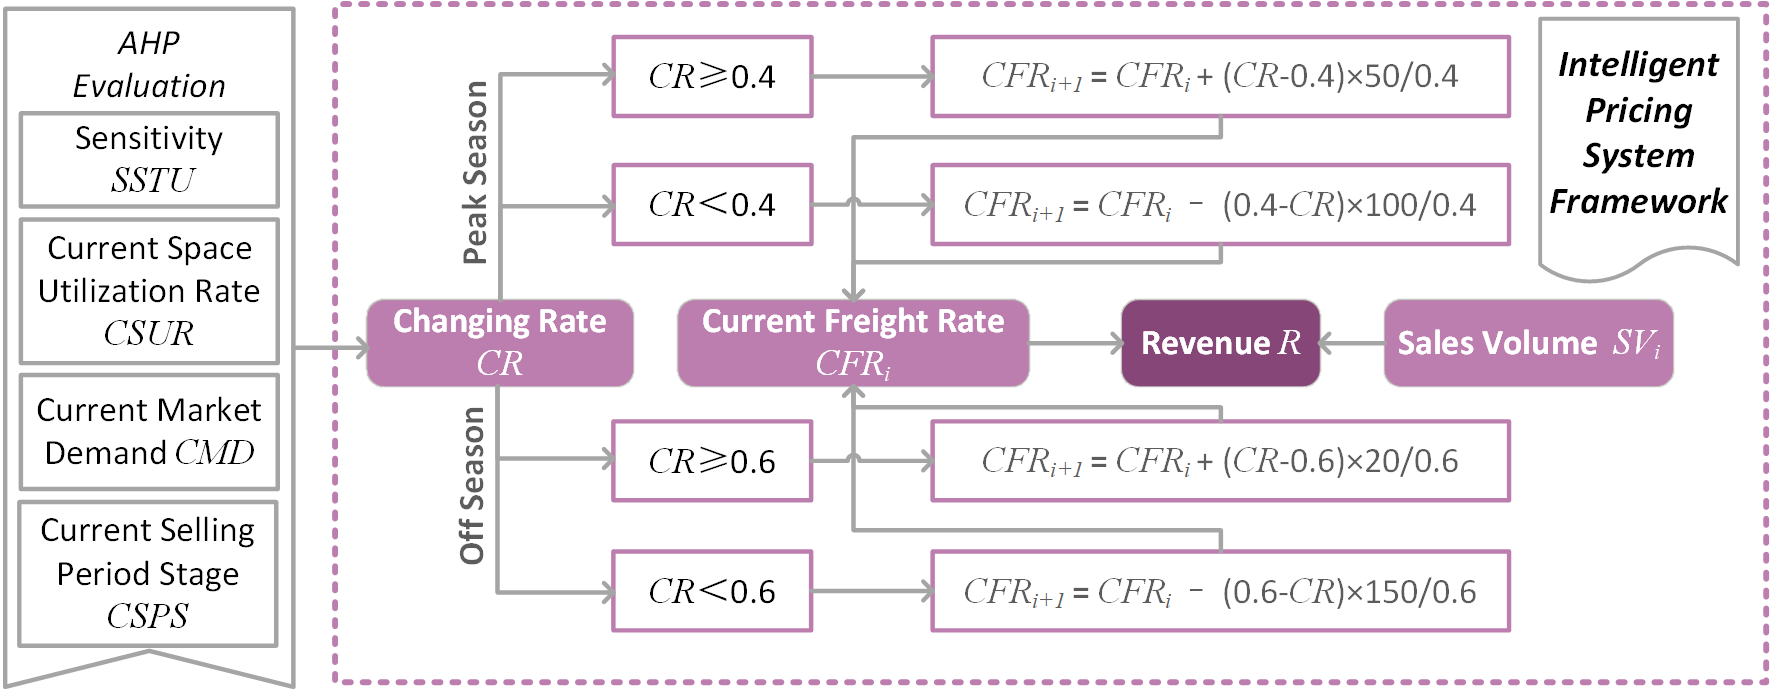
\includegraphics[scale=0.4]{Chapter-Mock/images-Mock/Intelligent Pricing System.png}
    \caption{Intelligent pricing system framework.}
    \label{fig:Intellignet pricing system}
\end{figure}

\item Rational Test

\hspace{1em}
Same as the former part 3.1, we do the rational test to the intelligent pricing strategy and get the following figure \ref{fig:Mock-Rationality-Intelligent}.

\begin{figure}[H]
    \centering
    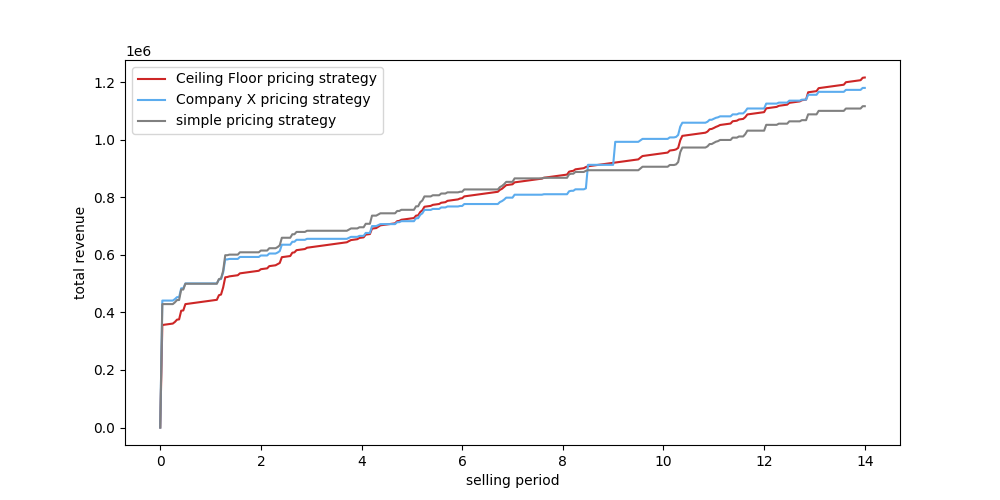
\includegraphics[scale=0.6]{Chapter-Mock/images-Mock/3_2.png}
    \caption{Rationality test of the intelligent pricing strategy.}
    \label{fig:Mock-Rationality-Intelligent}
\end{figure}

\hspace{1em}
We notice that the curve of the intelligent pricing strategy is increasing more smoothly and its revenue is slightly bigger than the one of the existing pricing strategy.From this we can draw our conclusion that the model we designed is superior to the existing pricing strategy.

\end{enumerate}